%\documentclass[handout,ignorenonframetext,red]{beamer}
\documentclass[ignorenonframetext,red]{beamer}
%\documentclass[class=article, a4paper]{beamer}
%\documentclass[handout]{beamer} %pour sortie papier


\usepackage[french]{babel}
\usepackage{pgf,pgfarrows,pgfn odes,pgfautomata,pgfheaps,pgfs hade}
\usepackage{amsmath,amssymb}
\usepackage[utf8]{inputenc}
\usepackage{stmaryrd}
\usepackage{url}


%\documentclass[svgnames,ignorenonframetext]{beamer}
%\usepackage{times}
\usepackage{listings}
\usepackage{amsmath,multicol}
\usepackage{verbatim}
%\usepackage{beamerarticle}
\usepackage{longtable}
%\usepackage{ucs}
%\usepackage[utf8]{inputenc}
\usepackage{pdfpages}

\setcounter{tocdepth}{1}

\mode<presentation>
{
  \usetheme{Warsaw}
  \setbeamercovered{transparent}
  \AtBeginSection[]
  {
    \begin{frame}<beamer>
       \setcounter{tocdepth}{2}
       \tableofcontents[currentsection,currentsubsection,hideothersubsections]
    \end{frame}
  }

  \AtBeginSubsection[]
  {
    \begin{frame}<beamer>
    \frametitle{\thesection. \insertsectionhead}
       \tableofcontents[sectionstyle=hide/hide,subsectionstyle=show/shaded/hide ]
    \end{frame}
  }
  
  \addtobeamertemplate{footline}{\insertframenumber/\inserttotalframenumber}

}

%\mode<handout>{  \setbeamercolor{background canvas}{bg=black!5}} }


\logo{\vspace{-.10cm} \includegraphics[scale=0.1]{../illustration/logo_cnam.png}}
\date{\today}
\author{Rémi LEBLOND\\ \url{http://remileblond.fr/SMB137}}
\institute{Conservatoire National des Arts et Métiers - Centre de Strasbourg}



\title{SMB137 - Cinquième partie}
\subtitle{Virtualisation de Systèmes}

\begin{document}
\frame[plain]{\titlepage}


\begin{frame}
 \frametitle{Plan}
 \tableofcontents
\end{frame} 

\section{Qu'est-ce que la virtualisation ?}

\subsection{Système virtuel}

\begin{frame}
\frametitle{Qu'est-ce que la virtualisation ?}
\begin{block}{Qu'est-ce qu'un composant virtuel ?}
\begin{itemize}
\item apparence fonctionnelle $\ne$ structure physique
\item mémoire, systèmes de fichiers... machine complète
\end{itemize}
\end{block}
\begin{itemize}
\item <2>Virtualisation de systèmes :
\begin{itemize}
\item fait fonctionner X systèmes sur Y machines physiques
\item généralement, $X \ne Y$
\end{itemize}
\item <3>Finalités
\begin{itemize}
\item maintenabilité
\item consolidation
\item souplesse
\end{itemize}
\end{itemize}
\end{frame}

\subsection{Usages de la virtualisation}

\begin{frame}
\frametitle{Historique}
\begin{itemize}

\item <1>En grande partie développé au centre scientifique de Cambridge d'IBM
\begin{itemize}
\item En collaboration avec le MIT
\item Mise au point du système expérimental CP/CMS
\item Devenu ensuite VM/CMS
\end{itemize}
\item <2>Commercialisé sur IBM OS/360
\begin{itemize}
\item 1965 : introduction du temps partagé
\item rétro-compatibilité par émulation des séries 1400 ou 7094 (logiciel et micro-code)
\item repris ensuite sur l'ensemble de la gamme mainframe
\end{itemize}
\item <3>Vers 1985-90 : virtualisation pour les ordinateurs personnels
\begin{itemize}
\item émulation de différents systèmes (ordinateur, consoles...)
\item support purement logiciel ou adossé à du matériel additionnel (processeur... )
\end{itemize}
\end{itemize}
\end{frame}

\begin{frame}{Historique}
\begin{exampleblock}{Exemples d'émulateurs sur ordinateurs personnels}
\begin{itemize}
\item Commodore Amiga à la pointe
\begin{itemize}
\item Processeurs hétérogènes : 80386 et 80486, 68xxx, et PPC
\item Possibilité de lancer d'autres systèmes d'exploitation
\begin{itemize}
\item Dos / Windows, Macintosh, Unix, Atari...
\end{itemize}
\end{itemize}
\item SideCar et PC Task sur PC
\item Emplant et ShapeShifter sur Macintosh
\end{itemize}
\end{exampleblock}
\begin{figure}
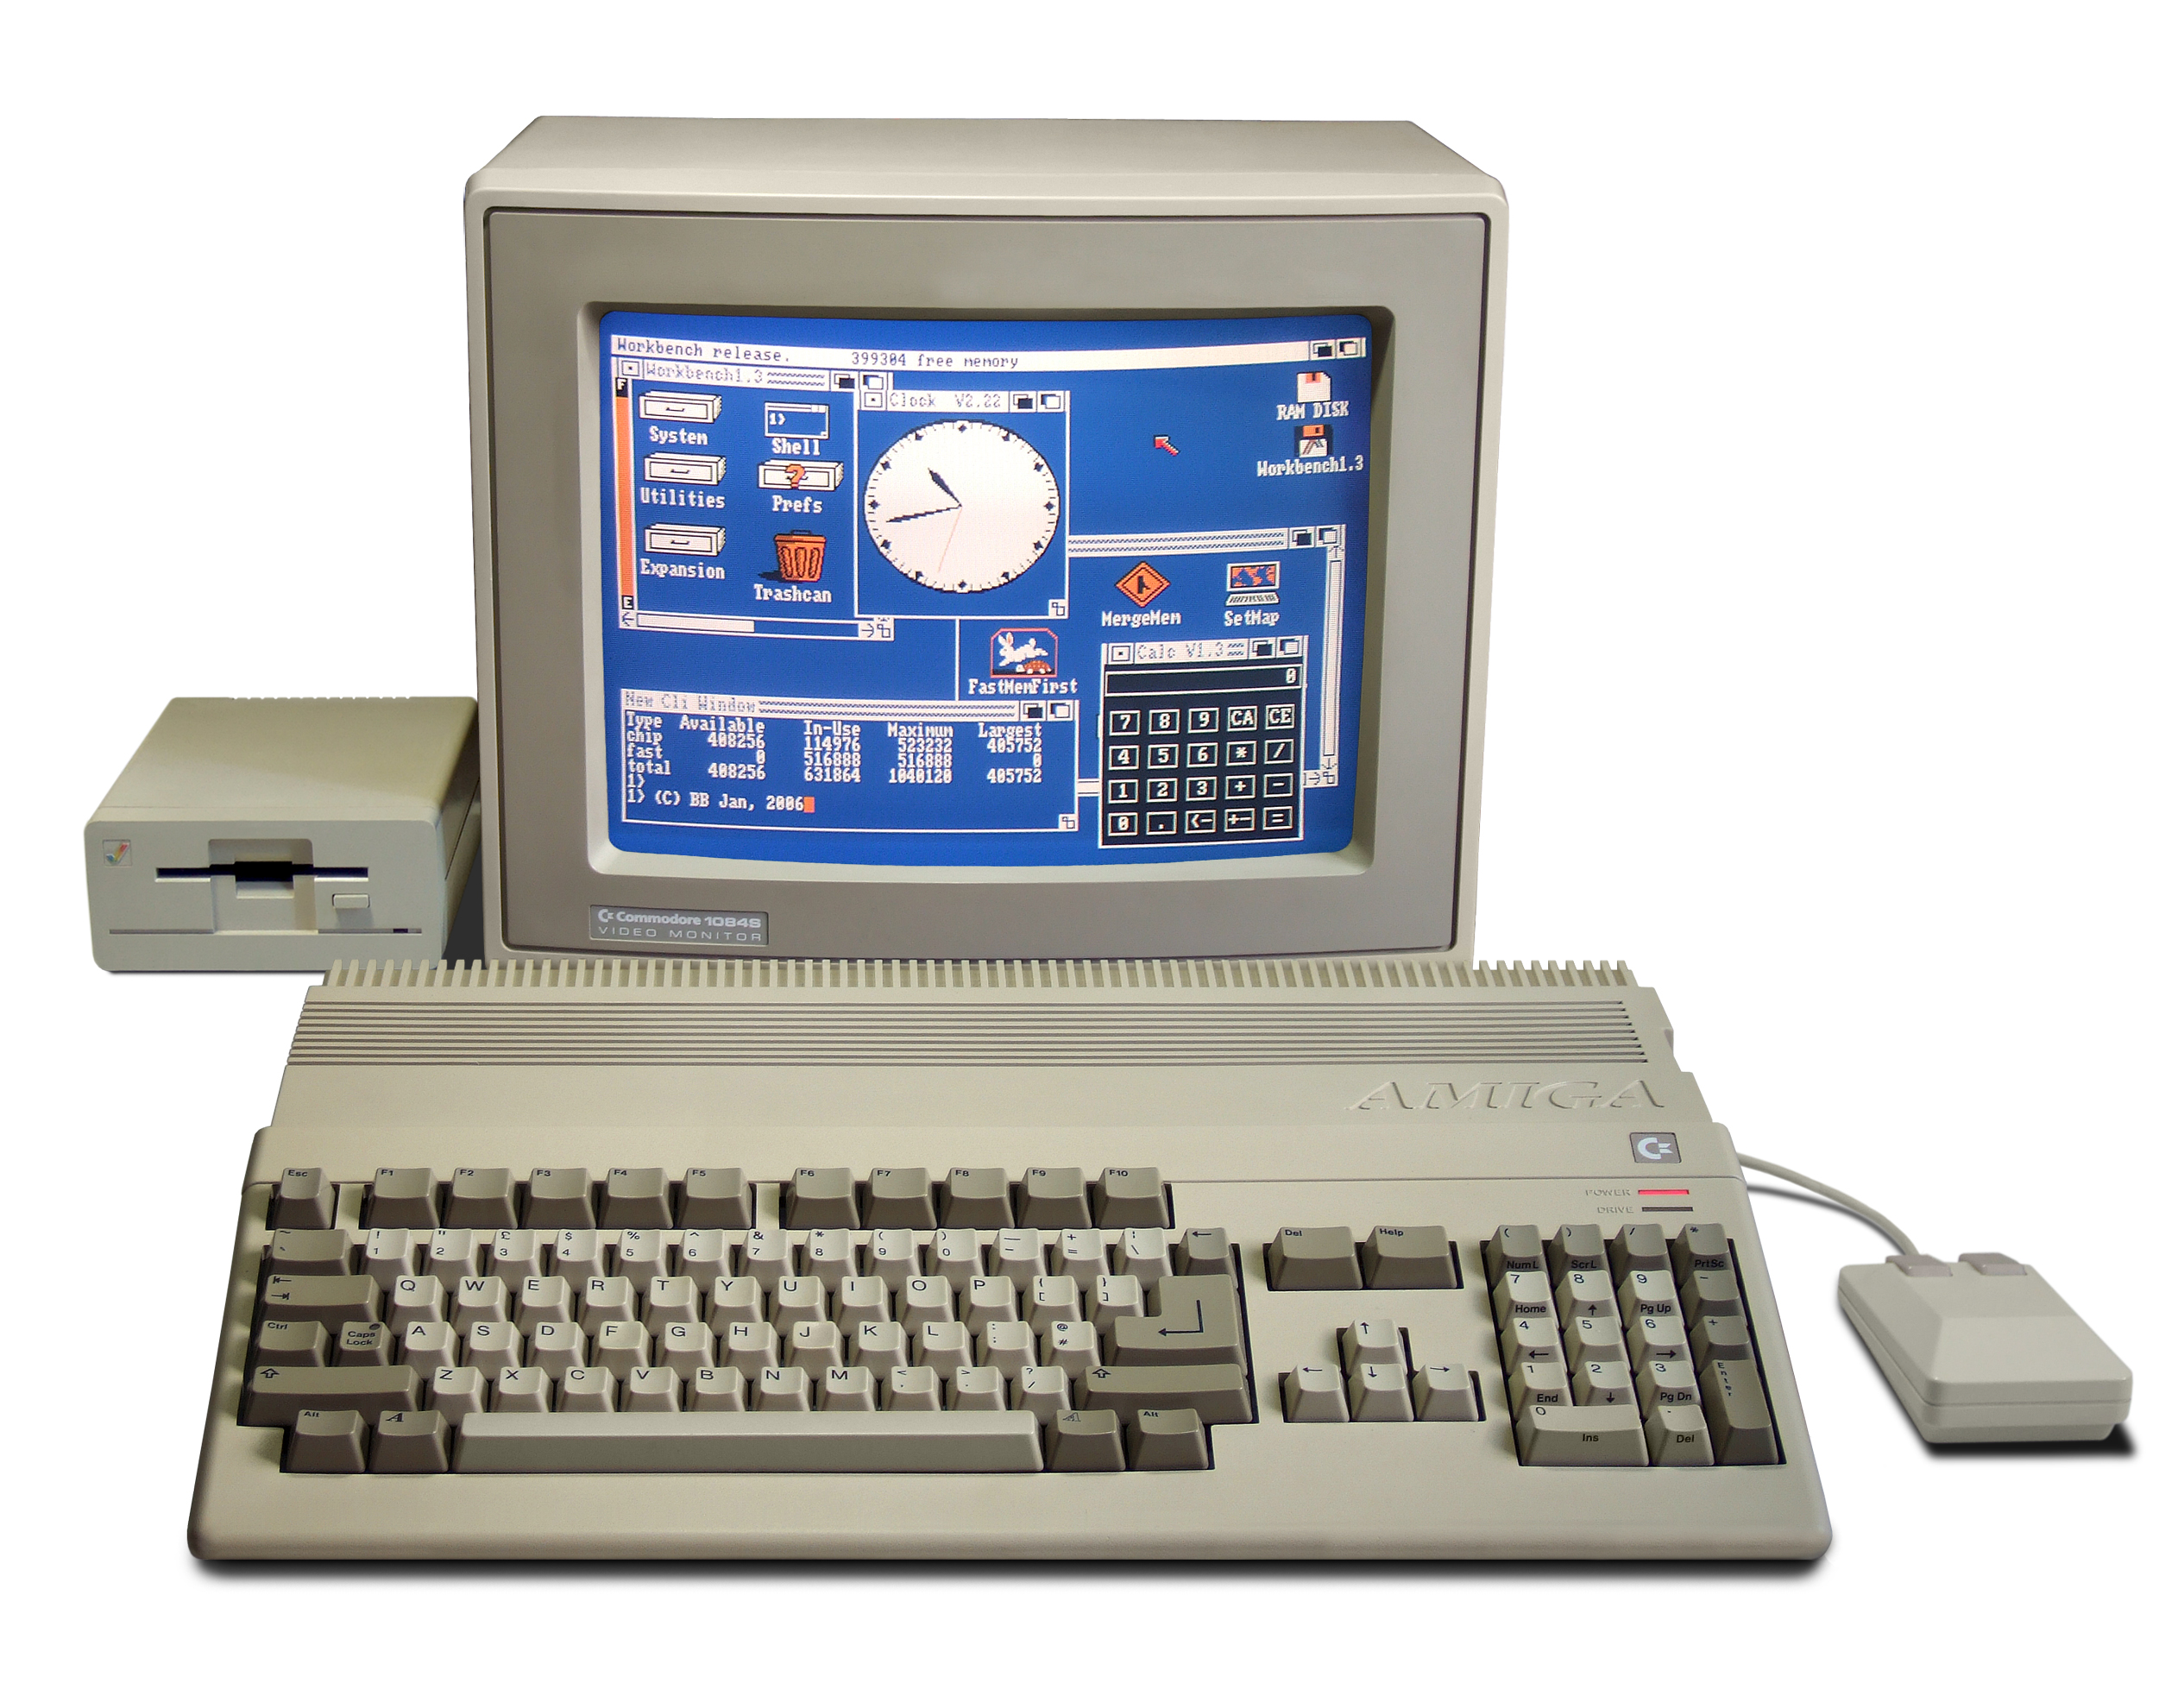
\includegraphics[height=2cm]{../illustration/Amiga500_system.jpg}
\caption{Amiga 500, 1987}
\end{figure}
\end{frame}

\begin{frame}
\frametitle{Historique}
\begin{itemize}
\item <1>Après 1990 : solutions Unix
\begin{itemize}
\item Architectures NUMA des Superdome d'HP (PA-RISC et IA-64)
\item E10000/E15000 de Sun (UltraSparc).
\end{itemize}

\item <2>Après 1995 : émulation de machines anciennes
\begin{itemize}
\item Atari, Amiga, Amstrad et les consoles NES, SNES, Neo-Geo AES
\end{itemize}

\item <3>Début 2000 : explosion des solutions de virtualisation professionnelles sur x86
\begin{itemize}
\item commerciales : VmWare en tête, VirtualPC, Virtual Server 
\item libres : Xen, KVM, QEMU, Bochs, Linux-VServer, Virtual Box
\end{itemize}
\end{itemize}

\end{frame}


\begin{frame}
\frametitle{Usages de la virtualisation}
\begin{itemize}

\item <1>Émulateur :
\begin{itemize}
\item VirtualPC, Parallels Desktop, Apple Rosetta
\end{itemize}

\item <2>Outil d'infrastructure :
\begin{itemize}
\item VmWare ESX, Microsoft Hyper-V Server, Citrix XenServer
\end{itemize}

\item <3>Support d'applications :
\begin{itemize}
\item JVM Java, CLR .Net
\end{itemize}

\end{itemize}
\end{frame}


\begin{frame}
\frametitle{Comparaison avec une architecture physique}
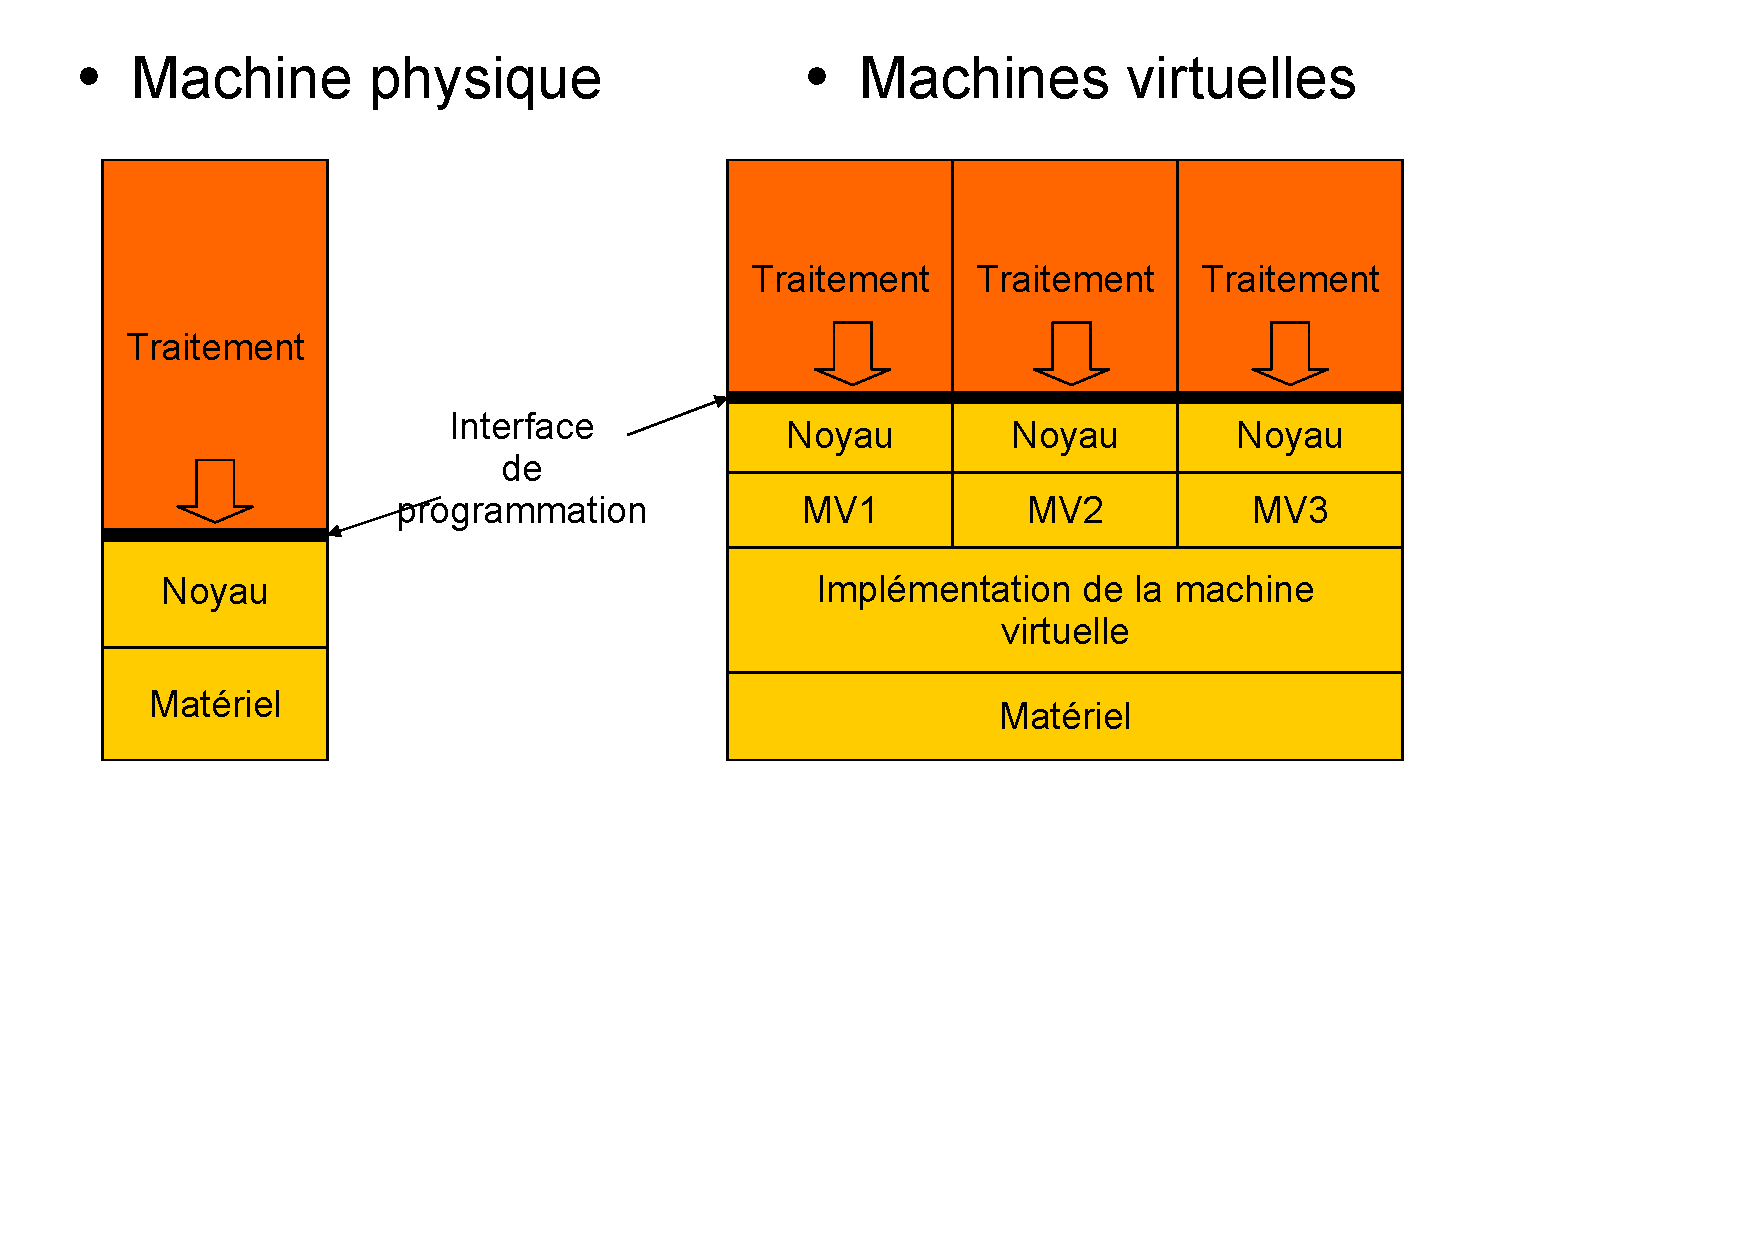
\includegraphics[height=6cm]{../illustration/compar_mp_mvirt.pdf}
\end{frame}

\begin{frame}
\frametitle{Exemple de combinaison de machines virtuelles}
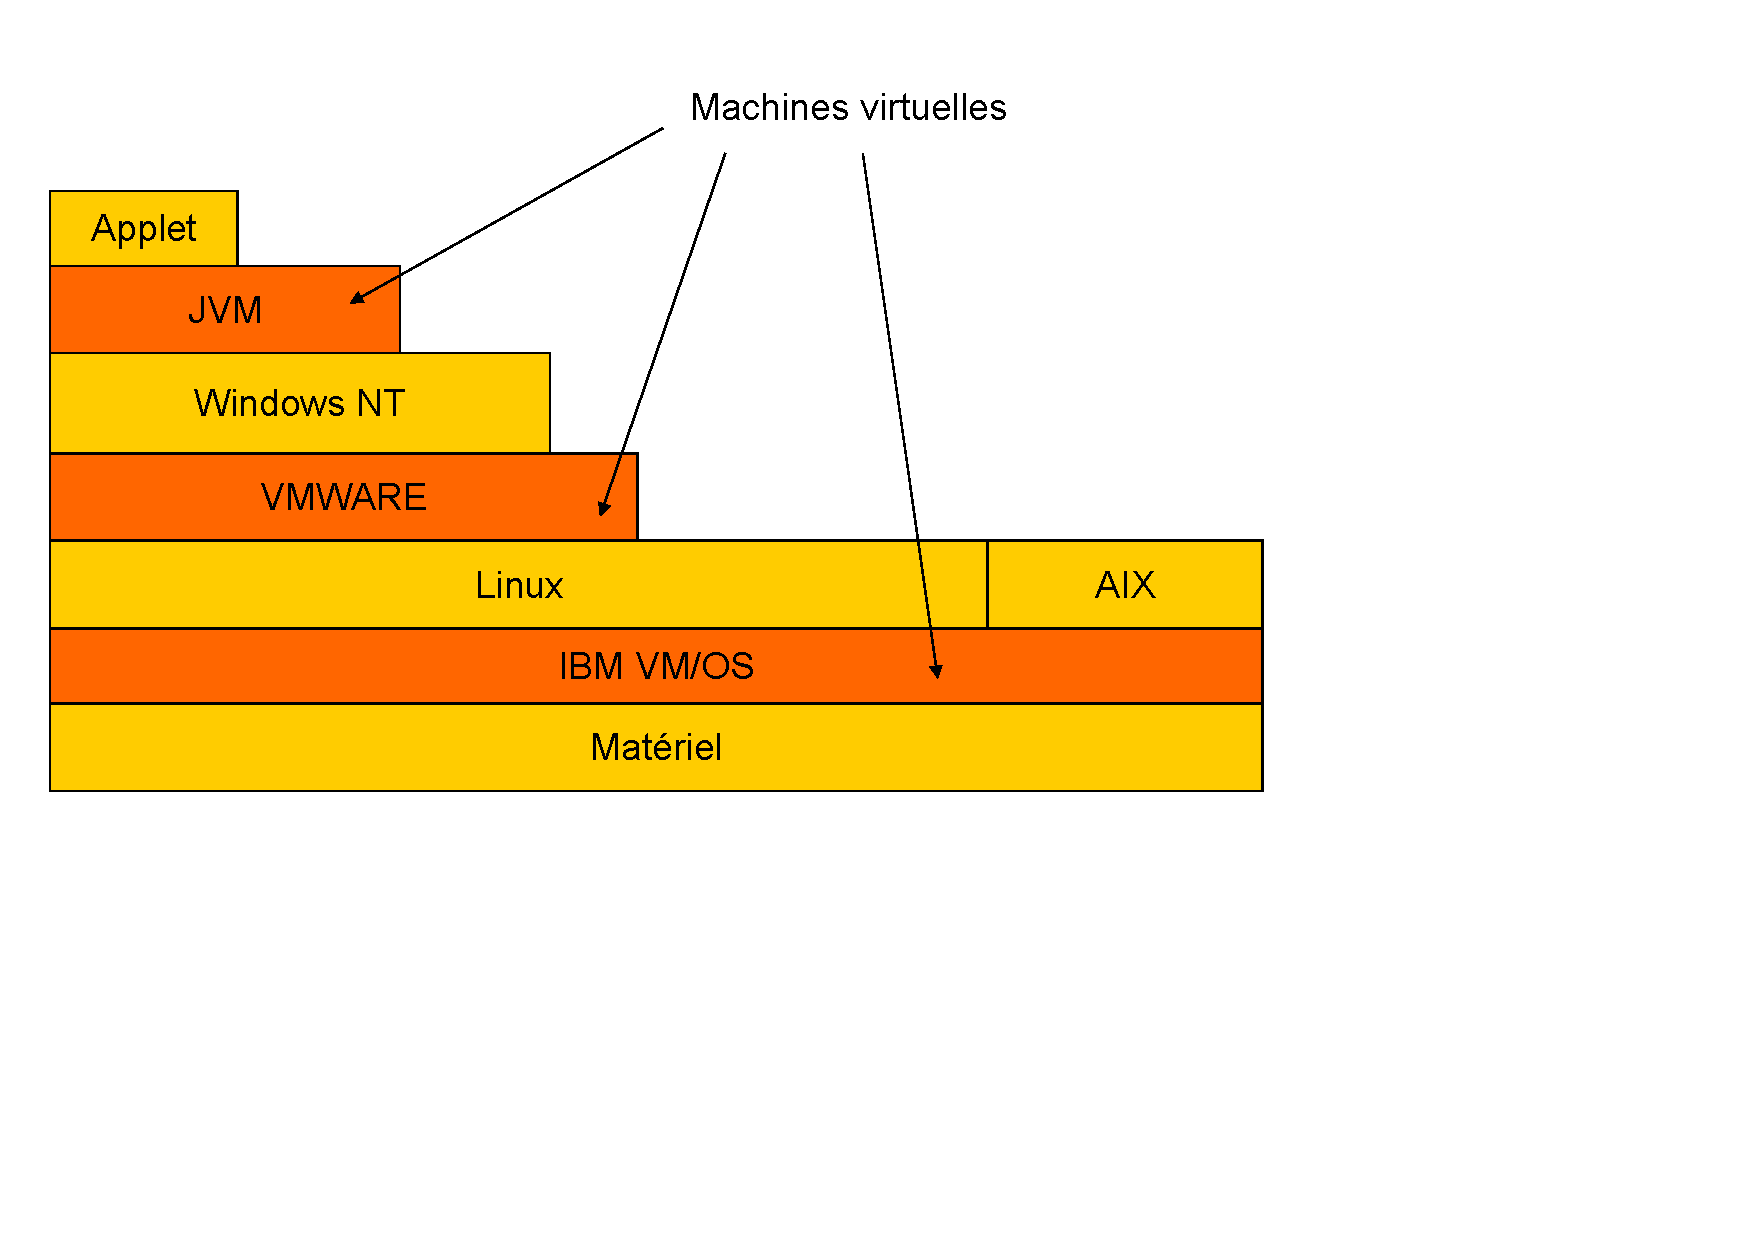
\includegraphics[height=6cm]{../illustration/exemple_mv.pdf}
\end{frame}

\subsection{Les intérêts de la virtualisation}

\begin{frame}
\frametitle{Pourquoi un tel essor ?}
\begin{itemize}
\item <1->Systèmes centraux
\begin{itemize}
\item concentration des centres de traitement
\end{itemize}

\item <2->Micro-informatique
\begin{itemize}
\item multiplication du nombre de serveurs
\item difficulté de maintenance
\item dépense énergétique
\end{itemize}

\item <3->Nécessité de re-centraliser
\end{itemize}

\begin{block}<4>{Trois problèmes}
\begin{itemize}
\item Sous-utilisation des ressources, adaptation aux besoins, équilibrage de charge
\item Difficultés de maintenance et de sécurisation
\item Moindre efficacité énergétique
\end{itemize}
\end{block}
\end{frame}

\begin{frame}
\frametitle{Intérêts de la virtualisation}
\begin{itemize}
\item <1->Utilisation optimale des ressources
\begin{itemize}
\item mutualisation du matériel
\item facilité d'adaptation à la charge
\item allocation dynamique des ressources
\end{itemize}
\item <2->Facilité d'installation, de gestion et de paramétrage
\begin{itemize}
\item réplication
\item points de reprise
\item plan de reprise/continuité facilités (PRA/PCA)
\end{itemize}
\item <3->Optimisation de la consommation énergétique
\end{itemize}
\end{frame}

\begin{frame}
\frametitle{Domaines d’application}
\begin{itemize}
  \item <1->Permet de mettre en place des serveurs virtuels dédiés (VDS)
   \begin{itemize}
  \item partage de ressource
  \item autonomie et le contrôle total du serveur
  \item hébergement mutualisé
\end{itemize}

\item <2->Améliore la disponibilité des serveurs ou des services
\begin{itemize}
  \item répartition de charge
\item reprise automatique sur incident

\end{itemize}
\item <3>Facilite les tests 
\begin{itemize}
  \item Simulation d'architectures complexes et hétérogènes
  \item Facilité de mise en œuvre
  \item Clonage et points de reprise
\end{itemize}

\end{itemize}
\end{frame}



\subsection{Critères d'évaluation}

\begin{frame}
\frametitle{Les critères d'évaluation de la virtualisation}
\begin{itemize}
\item La transparence
\begin{itemize}
\item Le fonctionnement du système non modifié par la virtualisation
\end{itemize}
\item Le cloisonnement
\begin{itemize}
\item fonctionnement indépendant
\item pas d'interférence entre machines virtuelles
\end{itemize}
\item Les performances
\begin{itemize}
\item minimisation des pertes liées à la virtualisation (overhead)
\end{itemize}
\end{itemize}
\end{frame}

\section{Les composants de la virtualisation}
\subsection{L'hyperviseur}

\begin{frame}
\frametitle{Implémentation de l'hyperviseur}
\begin{itemize}
\item Placé entre le matériel et le système d'exploitation
\item Utilisé pour les émulations de bas niveau
\item Implémentation :
\begin{itemize}
\item soit gère directement toutes les ressources (type 1)
\item soit hébergé par un système hôte (type 2)
\end{itemize}
\end{itemize}
\end{frame}

\begin{frame}
\frametitle{L'hyperviseur natif - type 1}
\begin{itemize}
\item Différents noms
\begin{itemize}
  \item hyperviseur de type 1
  \item hyperviseur natif
  \item émulation "bare metal"\note{Métal nu}
\end{itemize}
\item Noyau simplifié
\begin{itemize}
\item allégé
\item optimisé pour accueillir des OS invités
\end{itemize}
\item Support matériel de bas niveau :
\begin{itemize}
\item pas de support spécifique
\begin{itemize}
\item paravirtualisation
\end{itemize}
\item instructions de virtualisation matérielle (AMD-V et Intel-VT)
\begin{itemize}
\item Virtualisation complète
\end{itemize}
\end{itemize}
\end{itemize}
\end{frame}



\begin{frame}
\frametitle{Hyperviseur natif - type 1}
\framesubtitle{Cas de la gestion directe des ressources}
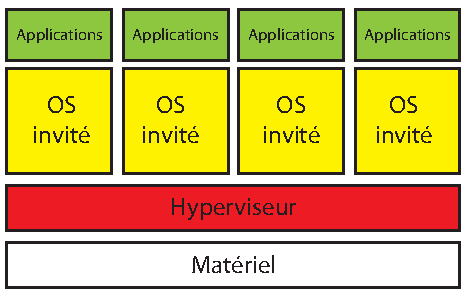
\includegraphics[width=0.8\textwidth]{../illustration/hyperviseur_natif.pdf}
\end{frame}

\begin{frame}
\frametitle{Hyperviseur natif}
\frametitle{Exemples de solutions - type 1}
\begin{exampleblock}{Solutions logicielles}
\begin{itemize}
\item CP/CMS d'IBM, ancêtre de z/VM
\item Xen (OpenSource), racheté par Citrix
\item Oracle VM
\item ESX Server de VMware
\item Hyper-V de Microsoft
\item Kernel-based Virtual Machine : QEmu / KVM (OpenSource)
\item Proxmox, OpenSource - Proxmox Server Solutions GmbH
\end{itemize}
\end{exampleblock}
\begin{exampleblock}{Solutions matérielles}
\begin{itemize}
\item Intégration de l'hyperviseur dans le micrologiciel (firmware)
\item Hyperviseur Virtage d'Hitachi
\end{itemize}
\end{exampleblock}
\end{frame}

\begin{frame}
\frametitle{Hyperviseur de type 2}
  \begin{itemize}
	  \item Logiciel qui s'exécute à l'intérieur d'un autre OS
	  \begin{itemize}
		    \item OS hôte
	  \end{itemize}
	  \item OS invité
	  \begin{itemize}
		  \item troisième niveau d'exécution au-dessus du matériel
		  \item perte de performance (overhead)
	  \end{itemize}
  \end{itemize}
  
\begin{exampleblock}{Exemples}
  \begin{itemize}
  \item VMware Server (ex GSX), Workstation, Fusion
  \item Open source QEMU
  \item Microsoft Virtual PC et VirtualServer
  \item VirtualBox d'Oracle
  \item Parallels Workstation de SWsoft et Parallels Desktop
\end{itemize}
\end{exampleblock}
\end{frame}


\begin{frame}
\frametitle{Hyperviseur de type 2}
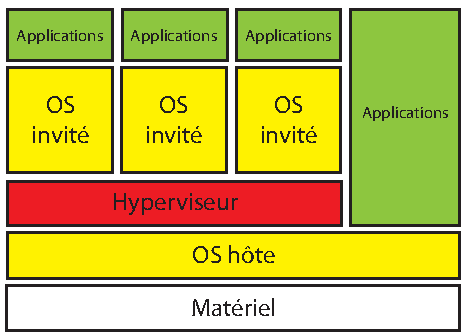
\includegraphics[width=0.8\textwidth]{../illustration/hyperviseur_invit.pdf}
\end{frame}

\begin{frame}
\frametitle{Hyperviseurs de type 1 ou 2}
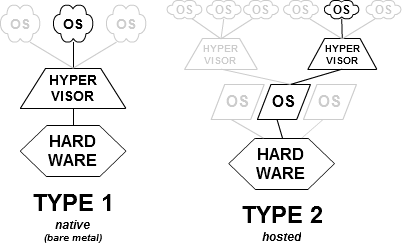
\includegraphics[width=0.8\textwidth]{../illustration/Hyperviseur.png}
\end{frame}


\subsection{L'émulateur}	

\begin{frame}
\frametitle{L’émulation du processeur}
\begin{itemize}
\item Simulation du processeur
\begin{itemize}
\item traduction de chaque instruction destinée à la CPU
\end{itemize}
\item Couteux en performances
\begin{itemize}
  \item émulation de très bas niveau
  \item overhead important
\end{itemize}
\item Viable uniquement si le système hôte et beaucoup plus puissant que le système invité :
\begin{itemize}
\item Atari, Playstation 1, Apple ][, GameBoy, Palm...
\end{itemize}
\end{itemize}
\end{frame}

\begin{frame}
\frametitle{L’émulation du processeur}
\begin{exampleblock}{Exemples de solutions}
\begin{itemize}
\item QEMU, émulateur OpenSource
\begin{itemize}
\item fonctionne ou émule x86, PPC ou Sparc
\end{itemize}
\item VirtualPC, racheté par Microsoft en 2003
\begin{itemize}
\item émulation d'un PC sur Mac PPC
\end{itemize}
\item Roseta, d'Apple
\end{itemize}
\end{exampleblock}
\end{frame}

\begin{frame}
\frametitle{Émulation d'un système hôte}
\begin{itemize}
\item Prise en charge d'une autre API, d'un autre format de fichier exécutable que le système cible
\item Impact beaucoup plus léger sur les performances
\begin{itemize}
\item Niveau d'abstraction nettement plus élevé
\end{itemize}
\end{itemize}
\begin{exampleblock}{Exemples} 
\begin{itemize}
\item Prise en charge de programmes Windows sur MacOsX ou Linux sur PC x86
\end{itemize}
\end{exampleblock}
\end{frame}

\begin{frame}
\frametitle{Émulation d'un système hôte}
\begin{exampleblock}{Wine} 
\begin{itemize}
\item Implémentation de l'API Win32
\begin{itemize}
\item Linux, MacOsX et autres Unix
\end{itemize}

\item Deux possibilités :
\begin{itemize}
\item Utilisation des DLL Windows 
\item Ré-écriture à partir des spécifications externes (logiciel libre)
\end{itemize}
\item Excellentes performances
\begin{itemize}
\item parfois meilleures que sous Windows
\item émulation de haut niveau
\item API système et non instructions processeur
\end{itemize}

\end{itemize}
\end{exampleblock}
\end{frame}

\subsection{Support matériel}


\begin{frame}
\frametitle{Support matériel}
\begin{itemize}
\item <1> Solutions matérielles :
\begin{itemize}
\item Intégration au processeur : 
\begin{itemize}
\item instructions spécifiques, niveaux de privilèges

\end{itemize}
\item Virtualisation des accès mémoire :
\begin{itemize}
\item MMU cloisonnables

\end{itemize}
\end{itemize}

\item <2> Aide au développement de systèmes virtualisés :
\begin{itemize}
\item Simplification de la virtualisation logicielle
\item Optimisation des performances
\item Doit nécessairement être exploité par du logiciel
\end{itemize}


\end{itemize}


\end{frame}

\begin{frame}
\frametitle{Support matériel}
\begin{exampleblock}{Exemples de support matériel}
\begin{itemize}
\item Hyperviseur IBM Power6 et Micro-partitionnement AIX
\item Mainframes : VM/CMS
\item Sun LDOM (hyperviseur pour la gestion de "logical domains")
\item Sun E10k/E15k
\item HP Superdome
\item AMD-V (anciennement Pacifica)
\item Intel VT (anciennement Vanderpool)
\end{itemize}
\end{exampleblock}
\end{frame}

\begin{frame}
\frametitle{Instructions dédiées à la virtualisation}
\begin{columns}
\column{0.7\textwidth}
\begin{itemize}
  \item Habituellement
  \begin{itemize}
  \item noyau en Ring 0
  \item programmes utilisateur en Ring 3
  \item seul l'OS hôte à accès au Ring 0
\end{itemize}
  \item <2->Technologie de partition processeur 
\begin{itemize}
  \item technologie de « décalage »
  \item géré par le BIOS
  \item OS invité exploite le Ring 2 lorsqu'il croit accéder au Ring 0
\end{itemize}
\end{itemize}

\begin{exampleblock}<3>{Implémentations}
\begin{itemize}
  \item VT-x (Virtual Technology) - 2003 - EPT (Extended Page Table) sur Nehalem
  \item AMD-V
\end{itemize}
\end{exampleblock}

\column{0.3\textwidth}
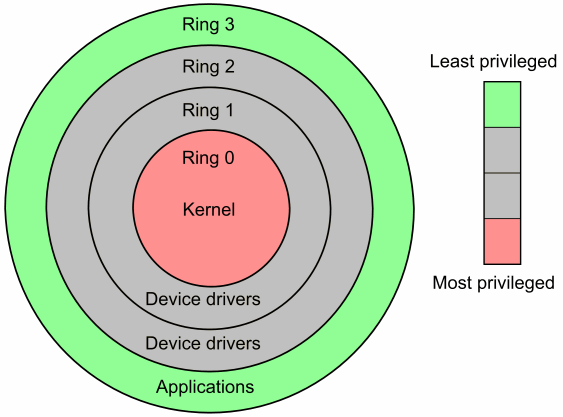
\includegraphics[width=7cm]{../illustration/cpu-ring-model.png}
\end{columns}
\end{frame}



\section{Les différentes approches de virtualisation}

\subsection{Isolation (cloisonnement)}

\begin{frame}
\frametitle{Le cloisonnement}
\begin{itemize}
\item <1->Partitionnement d’un système d'exploitation
\begin{itemize}
  \item tous les OS invités sont du même type
  \item isolés les uns des autres
\end{itemize}
\item <2->Séparation en plusieurs environnements
\begin{itemize}
\item tous sont régis par l'OS hôte
\item chaque processus ne peut interagir qu'avec les ressources et processus de son contexte
\end{itemize}
\item <3>Partionnement de serveurs
\end{itemize}
\end{frame}

\begin{frame}
\frametitle{Le cloisonnement}
\framesubtitle{Exemple d'Unix : \texttt{chroot}} 
\begin{itemize}
\item Isolement d'applications dans des contextes cloisonnés
\begin{itemize}
\item mini-système
\item accès limités
\item ne contient que les programmes et les ressources nécessaires
\end{itemize}
\item Utilisation d'un noyau unique
\item Solution légère à mettre en oeuvre (faible overhead)
\begin{itemize}
\item protection du système (serveur FTP, par exemple)
\item cohabitation d'applications incompatibles (bibliothèques)
\end{itemize}
\end{itemize}
\begin{exampleblock}{Exemple d'utilisation de \texttt{bash}}
\texttt{chroot /home/debian bash -i}
\end{exampleblock}
\end{frame}

\begin{frame}
\frametitle{Le cloisement}
\framesubtitle{Exemple de Linux VServer} 
\begin{columns}
\column{0.7\textwidth}

\includegraphics[width=3cm]{../illustration/VServer.png}
\begin{itemize}
\item Patch Linux + outils
\item Basé sur les Security Context
\begin{itemize}
\item serveurs virtuels Privés (VPS)
\item base utilisateurs propre
\item isolé de tous les autres VPS, mais partage les mêmes ressources matérielles
\end{itemize}
\item Permet d'exploiter de multiples systèmes sur un système hôte
\end{itemize}
\column{0.3\textwidth}
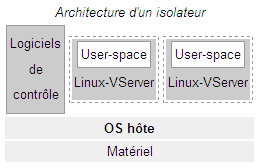
\includegraphics[width=4cm]{../illustration/VServer-archi.png}
\end{columns}
\end{frame}



\subsection{La paravirtualisation}

\begin{frame}
\frametitle{La paravirtualisation}
\begin{itemize}
\item Plus bas niveau que l'isolation
\item S’appuie sur une \emph{couche hyperviseur}
\begin{itemize}
\item bas niveau : interface avec les ressources matérielles
\item présente une machine générique spécifique
\item accueille des OS variés (invités)
\end{itemize}
\item <2>Nécessite une adaptation des systèmes invités
\begin{itemize}
\item OS modifié pour la paravirtualisation
\item interfaces spéciales $\rightarrow$ drivers
\item adaptation du système hôte et des systèmes invités
\end{itemize}
\end{itemize}
\end{frame}

\begin{frame}
\frametitle{La paravirtualisation}
\framesubtitle{Exemple de KVM / Virtio}
\begin{itemize}
\item Virtual Input-Output
\begin{itemize}
\item branche officielle du noyau Linux
\item OS invité : module du noyau Linux
\item OS hôte : outils spécifiques (Linux et Windows)
\end{itemize}
\item Pilote spécifique
\begin{itemize}
\item Traduit les demandes d'E/S en appel de haut niveau
\item ajout dans une liste FIFO exploitée par le système hôte
\item Support cartes réseau et contrôleurs de disques
\end{itemize}
\item Nécessite une adaptation du système invité
\begin{itemize}
\item uniquement pour des OS ouverts
\item Linux
\end{itemize}
\end{itemize}
\end{frame}


\subsection{La virtualisation complète}

\begin{frame}
\frametitle{La virtualisation complète}
\begin{itemize}
\item Hyperviseur de bas niveau
\begin{itemize}
\item émulation du niveau matériel
\item aucune modification de l'OS invité
\item transparence
\begin{itemize}
\item les OS invités n'ont pas conscience d'être virtualisés
\end{itemize}
\end{itemize}
\end{itemize}
\end{frame}

\section{Application de la virtualisation}

\subsection{Virtualisation de serveurs}

\begin{frame}
\frametitle{Virtualisation de serveurs}
\begin{itemize}
\item Utilisation traditionnelle de la virtualisation
\begin{exampleblock}{Exemples de solutions}
\begin{itemize}
\item Microsoft Hyper-V Server
\item VMWare vSphere Hypervisor (anciennement ESXi)
\item Citrix XenServer
\item Oracle VM Server
\item Proxmox VE
\end{itemize}
\end{exampleblock}
\end{itemize}
\end{frame}

\begin{frame}
\frametitle{Exemple}
\framesubtitle{Proxmox Virtual Environment}

\includegraphics[width=3cm]{../illustration/proxmox_logo.png}
\begin{itemize}
\item Solution libre de virtualisation
\item Virtualisation "bare metal"
\begin{itemize}
\item containers Linux (OpenVZ)
\item paravirtalisation (KVM / Virtio)
\item virtualisation complète (KVM\note{Kernel-based Virtual Machine} sur Intel-VT ou AMD-V)
\end{itemize}
\item Inclut :
\begin{itemize}
\item système d'exploitation complet (Debian Lenny 64 bits)
\item partitionnement de disque dur avec LVM2
\item outil de sauvegarde 
\item support du clustering avec migration à chaud des VM
\item outil Web d'administration et de surveillance
\end{itemize}
\end{itemize}
\end{frame}

\subsection{Virtualisation du poste client (VDI)}

\begin{frame}{Virtualisation du poste client}
VDI : Virtual Desktop Infrastructure :
\begin{itemize}
\item H-VDI : Hosted VDI :
\begin{itemize}
\item Hyperviseur centralisé
\item Client léger
\item Déport d'affichage (RCP, ICA)
\end{itemize}

\item Local-VDI : Hyperviseur local
\end{itemize}
\end{frame}

\subsection{Virtualisation d'application}

\begin{frame}
\frametitle{Virtualisation d'application}
\begin{itemize}
\item Emulation de plateforme : 
\begin{itemize}
\item Wine : émulation d'application Windows sur Linux
\item JVM, CLR : machine virtuelle Java/.Net
\end{itemize}
\item Encapsulation :
\begin{itemize}
\item  VMware ThinApp
\item Microsoft APP-V
\item Citrix XenApp
\end{itemize}
\item Conteneur d'application :
\begin{itemize}
\item Docker
\end{itemize}

\end{itemize}
\end{frame}

\begin{frame}
\frametitle{Conteneur d'application : Docker}
\begin{figure}[htbp]
   \centering
   
\includegraphics[height=1cm]{../illustration/docker-logo.png} 
   \caption{Logo de Docker}
   \label{fig:example}
\end{figure}
\begin{itemize}
\item Conteneurs applicatifs \cite{docker}
\item Abstraction de l'OS $\rightarrow$ gestion des ressources nécessaires
\end{itemize}
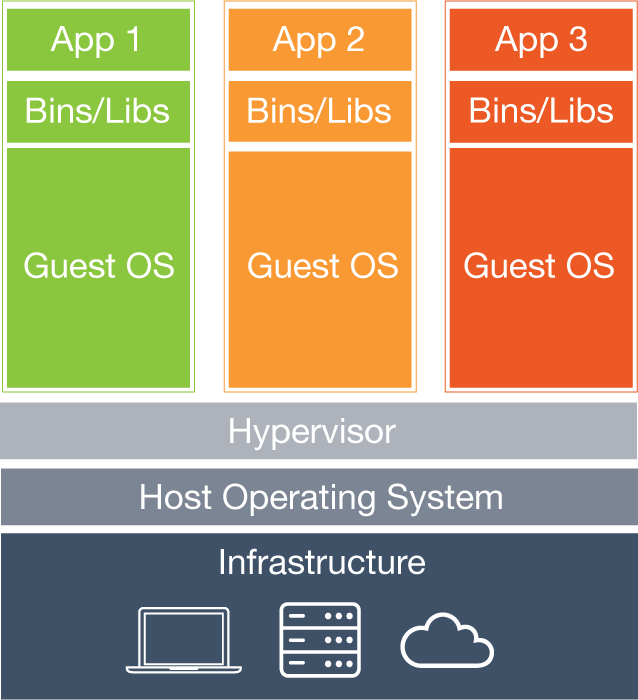
\includegraphics[height=3cm]{../illustration/docker-vm.png}
$\rightarrow$
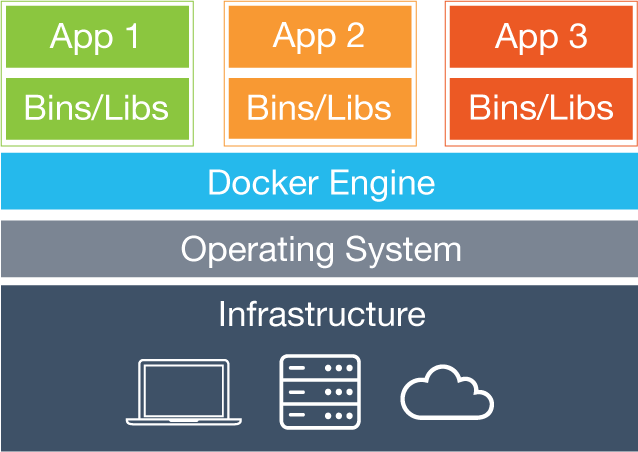
\includegraphics[height=3cm]{../illustration/docker-contener.png}
\end{frame}

\begin{frame}
\frametitle{Conteneur d'application : Docker}
\begin{figure}[htbp]
   \centering
   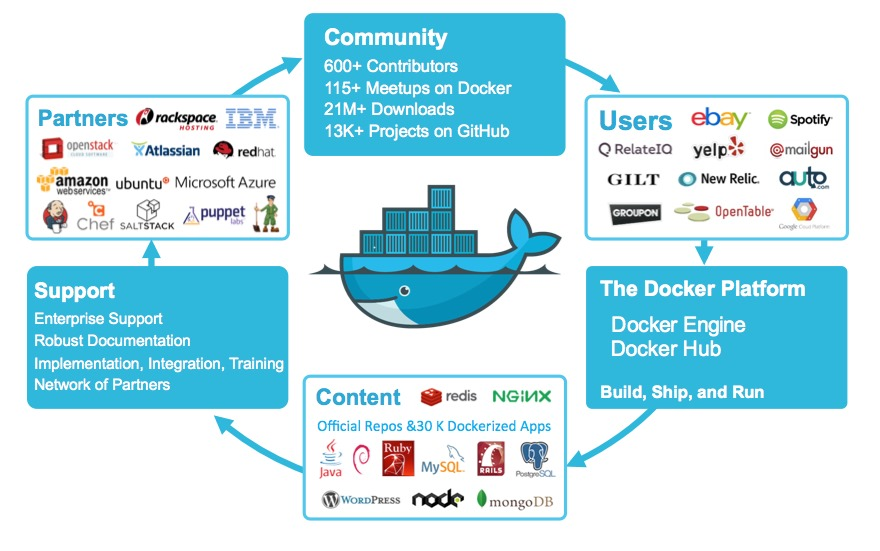
\includegraphics[height=6cm]{../illustration/docker-hub.jpg}
   \caption{L'écosystème Docker}
   \label{fig:example}
\end{figure}
\end{frame}

\begin{frame}
\frametitle{AuFS : union de systèmes de fichiers\cite{AuFS}}
\begin{itemize}
\item AuFS : Another Union File System
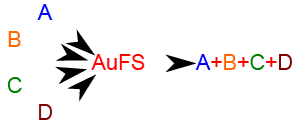
\includegraphics[height=2cm]{../illustration/AuFS.png}
\item implémenté sur la base d’UnionFS (Union File System)
\item rendre accessible au travers d’un montage la superposition, l’union, de plusieurs répertoires

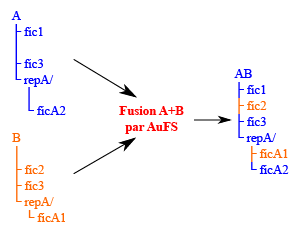
\includegraphics[height=2cm]{../illustration/AuFS-Exemples.png}
\end{itemize}

\end{frame}

\begin{frame}
\frametitle{Le Hub Docker}
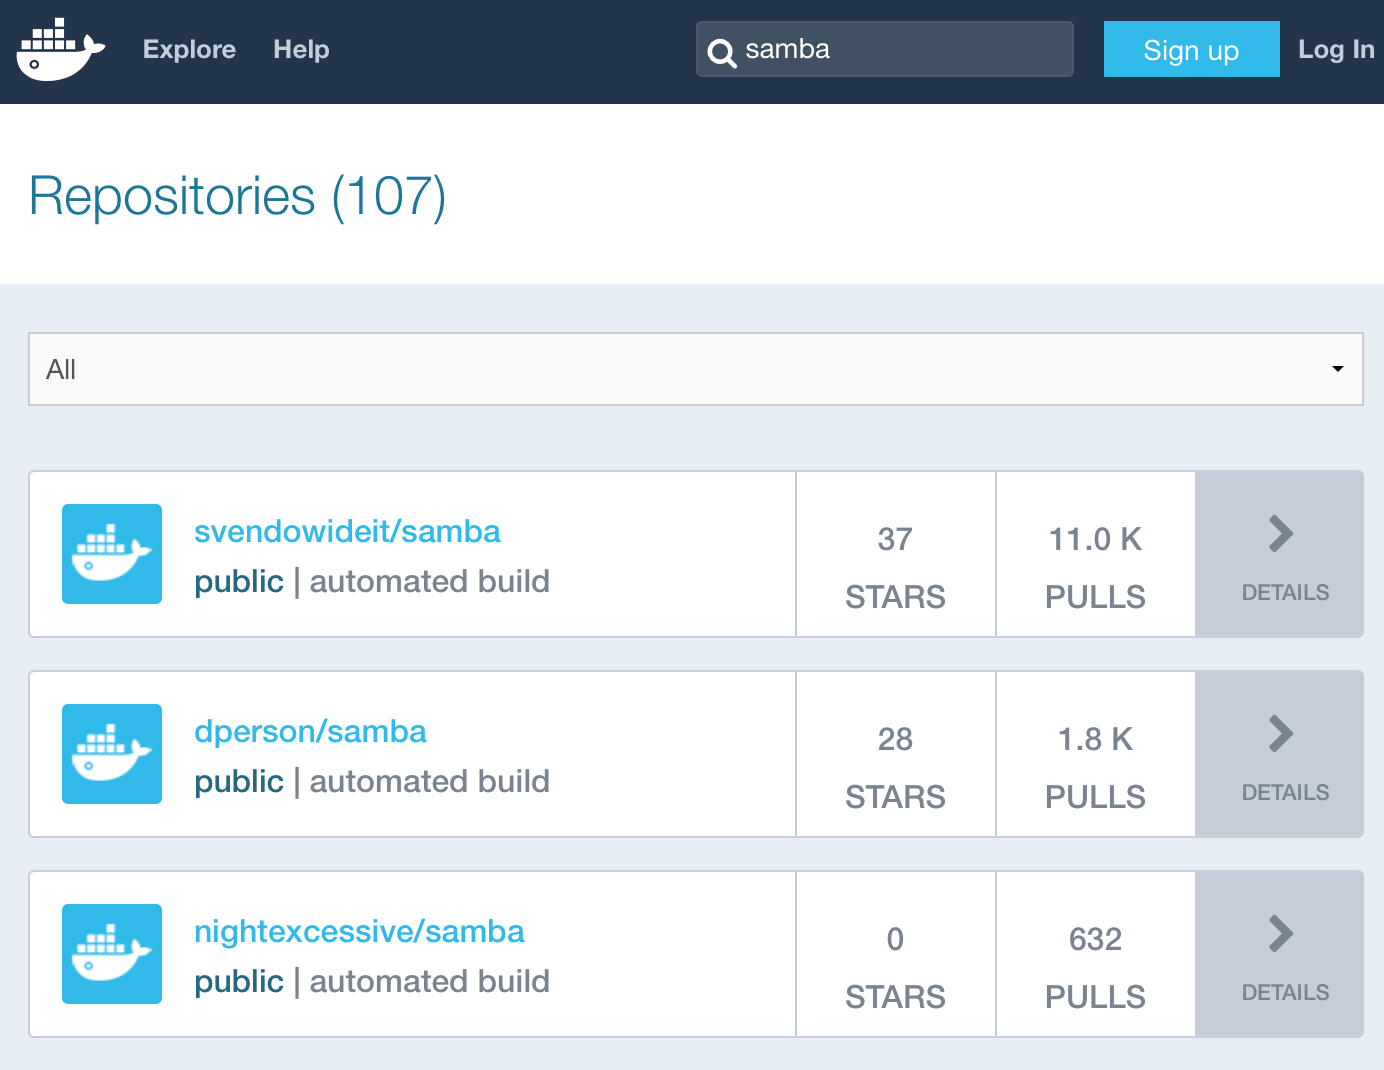
\includegraphics[height=6cm]{../illustration/DockerHub.png}
\end{frame}

\begin{frame}
\frametitle{Conteneur d'application : Docker}
\begin{itemize}
\item Lancer un système Debian avec une commande interactive (shell) :

\texttt{docker run -ti debian}
\item Lancer un système Debian avec redirection du répertoire \texttt{/root} : 

\texttt{docker run -ti -v /Users/remi/debian/:/root debian}
\item Lancer un système Debian en service, avec redirection du port 80 sur 8080 :

\texttt{docker run -ti -p 8080:80 -v /Users/remi/debian/:/root debian}
\end{itemize}
\end{frame}

\begin{frame}
\frametitle{Infrastructure as code : le Dockerfile}
\verbatiminput{../illustration/docker/Dockerfile}

\end{frame}

\begin{frame}
\frametitle{Docker compose}
\verbatiminput{../illustration/docker/docker-compose.yml}
\end{frame}

\subsection{Virtualisation et Cloud Computing}

\begin{frame}
\frametitle{Les cinq caractéristiques du Cloud Computing \cite{intro-cloud}}
\begin{enumerate}
\item <1>Accès réseau universel
\begin{itemize}
\item Accessible via le réseau, quel que soit le terminal
\end{itemize}
\item <2>Mise en commun de ressources
\begin{itemize}
\item \textit{pooling} des ressources logiques (puissance de calcul, capacité de stockage, bande passante disponible)
\item ne tient pas compte des ressources physiques (nombre de serveurs, taille de disques ou nombre de processeurs)
\end{itemize}
\item <3>Elasticité
\begin{itemize}
\item Possibilité d'adapter rapidement les ressources à ses besoins, dans un sens comme dans l'autre
\end{itemize}
\item <4>Libre-Service
\begin{itemize}
\item Traitement automatique des demandes de ressources
\end{itemize}
\item <5>Service mesurable et facturable
\begin{itemize}
\item facturation à l'usage, en fonction de la consommation de ressources
\end{itemize}
\end{enumerate}
\end{frame}

\begin{frame}
  \frametitle{Les différents niveaux de prise en charge}
  \begin{itemize}
  \item <1>[SaaS] : Software as a Service
  \begin{itemize}
  \item Mise à disposition d'applications
  \end{itemize}
  \item <2>[PaaS] : Platform as a Service
  \begin{itemize}
  \item Mise à disposition de plateformes de haut niveau
  \end{itemize}
  \item <3>[IaaS] : Infrastructure as a Service
  \begin{itemize}
  \item Mise à disposition d'une infrastructure virtuelle complète
  \end{itemize}
  \end{itemize}
\end{frame}

\begin{frame}
  \frametitle{Les différents niveaux de prise en charge \cite{intro-cloud}}
  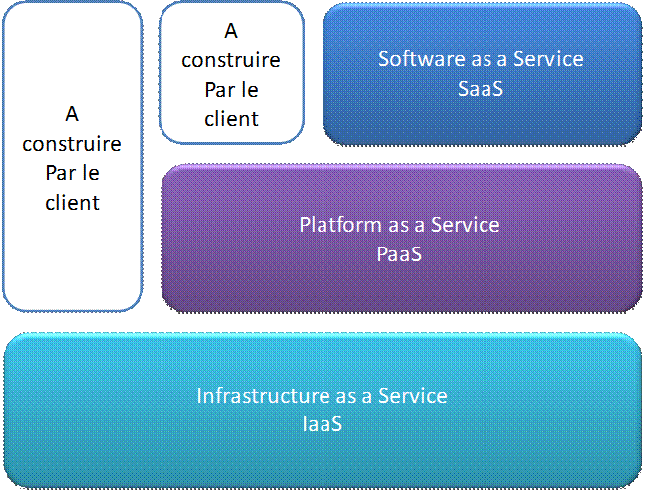
\includegraphics[height=7cm]{../illustration/niveaux-cloud.png}       
\end{frame}

\begin{frame}
\frametitle{SaaS : Software as a Service \cite{wp-saas}}
\begin{itemize}
\item Logiciel consommé sous la forme d’un service
\item Aucune visibilité sur la plateforme et l'infrastructure mises en oeuvre
\item Niveau d'abstraction : l'application
\end{itemize}
\begin{exampleblock}{Exemples de fournisseurs}
Google Docs, Office 365, Sales Force, Adobe Creative Cloud, Apple iCloud, DropBox, ... 
\end{exampleblock}
\end{frame}

\begin{frame}
\frametitle{PaaS : Platform as a Service}
\begin{itemize}
\item Mise à disposition d'une plateforme sur laquelle des développeurs peuvent déployer des applications
\item Exemples : 
\begin{itemize}
\item Serveur d'application (J2EE...), serveur Web, API...
\item Serveur de base de données (SQL, NoSQL... )
\end{itemize}
\item Niveau d'abstraction : la plateforme
\end{itemize}
\begin{exampleblock}{Exemples de fournisseurs}
Google App Engine (serveurs Google ou AppScale), Microsoft Azure...
\end{exampleblock}
\end{frame}

\begin{frame}
\frametitle{IaaS : Infrastructure as a Service}
\begin{itemize}
\item L'entreprise gère : 
\begin{itemize}
\item les systèmes d'exploitation des serveurs
\item les logiciels applicatifs (exécutables, paramétrages, l'intégration SOA, les bases de données)
\end{itemize}
\item Le fournisseur Cloud gère :
\begin{itemize}
\item le matériel serveur
\item les couches de virtualisation
\item le stockage
\item les réseaux
\end{itemize}
\item Niveau d'abstraction : l'infrastructure logique
\end{itemize}
\begin{exampleblock}{Exemples de fournisseurs}
Cloud Power, Desktone, Infoserv, Provectio, DotRiver...
\end{exampleblock}
\end{frame}

\begin{frame}
  \frametitle{Exemple d'IaaS : OpenStack}
  \begin{itemize}
  \item Plateforme OpenSource
  \begin{itemize}
    \item double licence GPL, LGPL
  \end{itemize}

  \item Compatible avec de nombreux hyperviseurs
  \begin{itemize}
    \item KVM, Xen, VmWare...
  \end{itemize}

  \item Soutenu par de nombreux acteurs importants
  \begin{itemize}
  \item NASA, IBM, Dell, HP, Cisco, NTT, Redhat, Canonical...
  \end{itemize}
  \end{itemize}
  
\includegraphics[height=3cm]{../illustration/logo-openstack.png}       
\end{frame}

\begin{frame}
  \frametitle{OpenStack : les composants de base}
  \begin{itemize}
  \item OpenStack Compute :
\begin{itemize}
\item gestion de l'exécution
\item communications réseau
\end{itemize}

  \item OpenStack Object Storage : \begin{itemize}
\item gestion du stockage des données
\end{itemize}

  \item OpenStack Image Service : \begin{itemize}
\item gestion des images de référence des machines virtuelles
\item image de base et snapshot
\end{itemize}

  \end{itemize}
\end{frame}

\frame[allowframebreaks]
{
\frametitle{Bibliographie}
\bibliographystyle{plain}
\bibliography{include/smb137}
}

\end{document}
